% ---
% Capitulo Tratamento dos Dados
% ---
\chapter{Tratamento dos Dados}\label{chap:trat-dados}

\section{Preparação da base de dados}\label{sec:bd-prep}

Afim de tornar possível comparar dados das diversas Pesquisas OD objetos deste trabalho (1977, 1987, 1997 e 2007) foi necessário conhecer o banco de dados de cada edição, e para que seja possível analisar a evolução de padrões de mobilidade e de comportamento, é preciso que os dados dos diversos bancos sejam comparáveis. Para isso, foi desenvolvido o desenho de um Banco de Dados Unificado (BDU), com função de integrar e compatibilizar as informações julgadas relevantes até este momento, e também aquelas que acredita-se possam vir a ser úteis em etapas posteriores do trabalho. Os \emph{layouts} dos bancos de dados originais podem ser observados no Anexo \ref{chap:anexo_layouts}, e o do banco integrador pode ser visto no Quadro \ref{qua:layout-haydee} a seguir.

Inicialmente, nos bancos de dados originais, foram identificadas as variáveis correspondentes entre os diversos anos e o BDU. Para cada variável e para cada ano foram feitas transformações para que fosse possível gerar um único banco de dados final, possível de ser empilhado - essas transformações estão descritas no Capítulo \ref{chap:trat-dados}. Devido ao tamanho dos bancos de dados, a preparação dos dados não foi feita em planilhas eletrônicas convencionais, mas por meio de códigos em linguagem \textit{python}. A estrutura dos códigos apresentados no Anexo \ref{chap:anexo_rotinas} é dividida em 5 blocos: (i) \textit{Set up} inicial com chamadas de bibliotecas e configurações; (ii) Definição de \textit{loggers}; (iii) Definição de funções gerais; (iv) Definição da função principal; e (v) Chamada para execução da função principal.\\ 

\begin{compactitem}[]
\item (i) \textit{Set up}: foram utilizadas as bibliotecas \textit{math}, para as funções matemáticas, e \textit{pandas}, as análises de dados.\\

\item (ii) Definição de \textit{loggers}\footnote{\textit{Logger} é uma rotina utilizada para acompanhar o processamento dos dados.}: foram estabelecidos dois \textit{loggers}, o \textit{log_output} que salva o conteúdo num arquivo de saída (de texto, com extensão .log) e o \textit{log_tela}, que além de salvar o conteúdo no arquivo de saída também mostra esse conteúdo na tela.\\

\item (iii) Definição de funções gerais: são definidas 5 funções gerais assessórias que serão utilizadas pelas funções gerais ``passo”. Ou seja, as 66 funções gerais ``passo'' são que, de fato, fazem o trabalho de transformação variável a variável. As assessórias servem para que estas possam ler os arquivos .csv e realizar testes de consistência, entre outras tarefas.\\

São funções gerais assessórias:
\item - consulta_refext: traz valor de referência externa (em arquivo csv) baseado em valor de referência do arquivo de origem;
\item - verifica_dummy: verifica se uma variável, do tipo \textit{dummy}, contém algum valor diferente de 0 ou de 1; 
\item - verifica_range: verifica se uma variável, do tipo número inteiro, contém algum valor fora de um intervalo especificado.
\item - corrige_renda: corrige a renda indicada aplicando um deflator que é passado como parâmetro; e
\item - coord: preenche as colunas de coordenadas ``CO_DOM_X'', ``CO_DOM_Y'', ``CO_ESC_X'', ``CO_ESC_Y'', ``CO_TRAB1_X'', ``CO_TRAB1_Y'', ``CO_TRAB2_X''; ``CO_TRAB2_Y'', ``CO_ORIG_X'', ``CO_ORIG_Y'', ``CO_DEST_X'' e ``CO_DEST_Y'', segundo consulta ao arquivo externo com correspondência entre subzonas e suas coordenadas x e y.\\

São funções gerais ``passo'':
\item - passo_ano: preenche a coluna ``ANO'' segundo as categorias do Quadro \ref{qua:layout-haydee};
\item - passo_dia_sem: preenche a coluna ``DIA_SEM'' segundo as categorias do Quadro \ref{qua:layout-haydee};
\item - passo_ucod: preenche a coluna ``UCOD'' segundo consulta ao arquivo externo com correspondência entre zonas e ucods;
\item - passo_zona_dom, passo_subzona_dom e passo_mun_dom: checa se existe algum erro no intervalo pertinente, respectivamente, às zonas, subzonas e municípios do domicílio de cada ano conforme Quadro \ref{qua:layout-haydee};
\item - passo_f_dom: checa se existe algum erro (número diferente de 0 ou 1) na coluna ``F_DOM'';
\item - passo_tipo_dom: checa se existe algum erro no intervalo pertinente aos tipos de domicílio conforme Quadro \ref{qua:layout-haydee};
\item - passo_f_fam: checa se existe algum erro (número diferente de 0 ou 1) na coluna ``F_FAM'';
\item - passo_cond_mora: faz transformações nas categorias da variável ``COND_MORA'' e checa se existe algum erro no intervalo pertinente à condição de moradia conforme Quadro \ref{qua:layout-haydee};
\item - passo_ren_fam: corrige a renda familiar segundo o parâmetro deflator passado pela função principal e armazena os valores na coluna ``REN_FAM'';
\item - passo_cd_renfam: faz transformações nas categorias da variável``CD_RENFAM'' e checa se existe algum erro no intervalo pertinente à renda individual conforme Quadro \ref{qua:layout-haydee};
\item - passo_f_pess: checa se existe algum erro (número diferente de 0 ou 1) em ``F_PESS'';
\item - passo_sit_fam:  faz transformações nas categorias da variável ``SIT_FAM'' e checa se existe algum erro no intervalo pertinente à situação familiar conforme Quadro \ref{qua:layout-haydee};
\item - passo_sexo: faz transformações nas categorias da variável ``SEXO'' de forma que seja uma \textit{dummy} que indica se pessoa é mulher ou não e checa se existe algum erro (número diferente de 0 ou 1);
\item - passo_grau_instr: faz transformações nas categorias da variável ``GRAU_INSTR'' e checa se existe algum erro no intervalo pertinente ao grau de instrução conforme Quadro \ref{qua:layout-haydee};
\item - passo_estuda: atribui \textit{dummy} que indica se pessoa estuda ou não, ou seja, se zona da escola for zero (0) então, pessoa não estuda (0), caso contrário, a pessoa estuda (1); além de checar se existe algum erro (número diferente de 0 ou 1);
\item - passo_ocup: faz transformações nas categorias da variável ``OCUP'' e checa se existe algum erro no intervalo pertinente à condição de ocupação da pessoa conforme Quadro \ref{qua:layout-haydee};
\item - passo_setor_ativ: faz transformações nas categorias da variável ``SETOR_ATIV'' e checa se existe algum erro no intervalo pertinente à condição de ocupação da pessoa conforme Quadro \ref{qua:layout-haydee}; 
\item - passo_ren_ind: corrige a renda familiar segundo o parâmetro deflator passado pela função principal e armazena os valores na coluna ``REN_IND'';
\item - passo_cd_renind: faz transformações nas categorias da variável ``CD_RENIND'' de forma que seja uma \textit{dummy} que indica se pessoa tem renda ou não e checa se existe algum erro (número diferente de 0 ou 1);
\item - passo_f_viag: checa se existe algum erro (número diferente de 0 ou 1) na coluna ``F_VIAG";
\item - passo_fe_viag: não se mexe na coluna ``FE_VIAG'';
\item - passo_zona_esc, passo_subzona_esc e passo_mun_esc: checa se existe algum erro no intervalo pertinente, respectivamente, às zonas, subzonas e municípios da escola de cada ano conforme Quadro \ref{qua:layout-haydee};
\item - passo_zona_trab1, passo_subzona_trab1 e passo_mun_trab1: checa se existe algum erro no intervalo pertinente, respectivamente, às zonas, subzonas e municípios do trabalho 1 de cada ano conforme Quadro \ref{qua:layout-haydee};
\item - passo_zona_trab2, passo_subzona_trab2 e passo_mun_trab2: checa se existe algum erro no intervalo pertinente, respectivamente, às zonas, subzonas e municípios do trabalho 2 de cada ano conforme Quadro \ref{qua:layout-haydee};
\item - passo_zona_orig, passo_subzona_orig e passo_mun_orig: checa se existe algum erro no intervalo pertinente, respectivamente, às zonas, subzonas e municípios da origem da viagem de cada ano conforme Quadro \ref{qua:layout-haydee};
\item - passo_zona_dest, passo_subzona_dest e passo_mun_dest: checa se existe algum erro no intervalo pertinente, respectivamente, às zonas, subzonas e municípios do destino da viagem de cada ano conforme Quadro \ref{qua:layout-haydee};
\item - passo_serv_pas_orig e passo_serv_pas_dest: atribui \textit{dummy} que indica se pessoa serve passageiro ou não transformando as categorias das variáveis ``SERV_PAS_ORIG'' e ``SERV_PAS_DEST'', respectivamente, e checa se existe algum erro no intervalo pertinente ao ato de servir passageiro conforme Quadro \ref{qua:layout-haydee};
\item - passo_motivo_orig e passo_motivo_dest: faz transformações nas categorias das variáveis ``MOTIVO_ORIG'' e ``MOTIVO_DEST'', respectivamente, e checa se existe algum erro no intervalo pertinente ao motivo conforme Quadro \ref{qua:layout-haydee};
\item - passo_modo1, passo_modo2, passo_modo3 e passo_modo4: faz transformações nas categorias das variáveis ``MODO1'', ``MODO2'', ``MODO3'' e ``MODO4'', respectivamente, e checa se existe algum erro no intervalo pertinente aos modos de transporte usados segundo o Quadro \ref{qua:layout-haydee};
\item - passo_modo_prin: faz transformações nas categorias da variável ``MODO_PRIN'' e checa se existe algum erro no intervalo pertinente ao principal modo de transporte usado segundo o Quadro \ref{qua:layout-haydee};
\item - passo_tipo_est_auto: faz transformações nas categorias da variável ``TIPO_EST_AUTO'' e checa se existe algum erro no intervalo pertinente ao principal modo de transporte usado segundo o Quadro \ref{qua:layout-haydee};
\item - passo_valor_est_auto: corrige o valor do estacionamento segundo o parâmetro deflator passado pela função principal e armazena os valores na coluna ``VALOR_EST_AUTO'', caso essa variável não existe, não se mexe na coluna e os valores serão tomados como \textit{NA};
\item - passo_no_dom: gera o número do domicílio sendo que para cada ``ZONA_DOM'' o ``NO_DOM'' será atualizado sempre que ``F_DOM'' for igual a 1; caso contrário, se ``F_DOM'' for igual a zero, então``NO_DOM'' será igual ao ``NO_DOM'' da linha anterior;
\item - passo_no_fam:  gera o número da família sendo que para cada ``ID_DOM'' o ``NO_FAM'' será incrementado sempre que ``F_FAM'' for igual a 1; caso contrário, se ``F_FAM'' for igual a 0, então
o ``NO_FAM'' será igual ao ``NO_FAM'' da linha anterior; 
\item - passo_no_pess: gera o número da pessoa sendo que para cada ``ID_FAM'' o ``NO_PESS'' será atualizado sempre que ``F_PESS'' for igual a 1; caso contrário, se ``F_PESS'' for igual a zero, então ``NO_PESS'' será igual ao ``NO_PESS'' da linha anterior;
\item - passo_no_viag: gera o número da viagem sendo que para cada ``ID_PESS'' o ``NO_VIAG'' começa com 1 e será incrementado sempre que ``F_VIAG'' for igual a 1; caso contrário, se ``F_VIAG'' for igual a 0, então o ``NO_VIAG'' será igual ao ``NO_VIAG'' da linha anterior. Para garantir a representatividade do caso em que as pessoas responderam o questionário e não realizaram viagem,   quando o ``FE_VIAG'' for não nulo e ``ZONA_ORIG'' e ``ZONA_DEST'' forem ambas nulas simultaneamente o ``NO_VIAG'' será igual a 0;
\item - passo_id_dom: gera o ``ID_DOM'' que é composto por 8 dígitos, em que o primeiro é o ano conforme Quadro \ref{qua:layout-haydee}, do segundo ao quarto dígitos tem-se a zona, e do quinto ao oitavo dígitos tem-se o número do domicílio;
\item - passo_id_fam: gera o ``ID_FAM'' que é composto por 10 dígitos, em que os 8 primeiros correspondem ao ``ID_DOM'' e os dois últimos ao ``NO_FAM''; 
\item - passo_id_pess: gera o ``ID_PESS'' que é composto por 12 dígitos, em que os 10 primeiros correspondem ao ``ID_FAM'' e os dois últimos ao ``NO_PESS''; 
\item - passo_id_viag: gera o ``ID_VIAG'' que é composto por 14 dígitos, em que os 12 primeiros correspondem ao ``ID_PESS'' e os dois últimos ao ``NO_VIAG'';
\item - passo_tot_viag: calcula e confere o campo ``TOT_VIAG'' baseado no máximo valor de ``NO_VIAG'' para cada pessoa;
\item - passo_cd_entre: substitui-se os valores da coluna “CD_ENTRE” segundo os valores de “TOT_VIAG”, considerando que todas entrevistas são consideradas "completas", segundo informação do Metrô.\\

\begin{figure}[htb]%
    \caption{\label{fig:id-esquema}Esquema indicativo da formação dos IDs}%
    \begin{center}%
        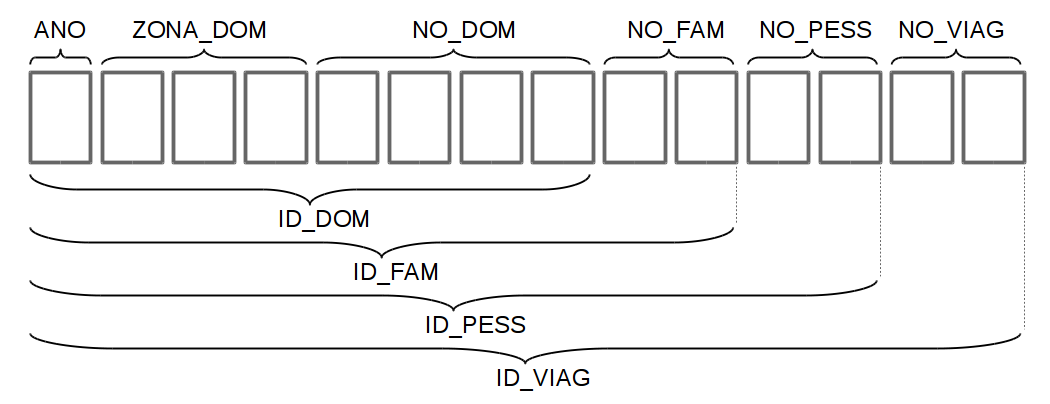
\includegraphics[width=0.75\textwidth]{./imagens/esquema-ID.png}%
    \end{center}%
%    \fonte{Elaboração própria}
\end{figure}%

\item (iv) Definição da função principal: principia lendo o banco de dados original (arquivo tipo OD__.csv) e também outros arquivos auxiliares de dados estruturados, como o ucod__.csv, o setor_ativ__.csv e o coord_subzonas__.csv – sendo um arquivo desses para cada OD analisada. Logo, temos 4 arquivos .csv principais de entrada e 12 auxiliares. O arquivo ucod__.csv contém a relação de cada zona e sua respectiva UCOD, o arquivo setor_ativ__.csv contém a relação de código do setor de atividade do banco original e o respectivo código no banco unificado. O arquivo coord_subzonas__.csv contém as coordenadas dos centroides das subzonas extraídos a partir dos arquivos de mapas e que não constavam originalmente do banco de dados. No caso de 1977, não se conseguiu o arquivo do MapInfo com a granularidade das subzonas, portanto, foram utilizadas as coordenadas dos centroides das zonas. Na sequência, As colunas que não existiam originalmente no banco de dados são geradas e reordenadas. Existe uma variável de controle (``passo'') que a cada passo executado incrementa 1. São chamadas as funções gerais. Vale notar que ficaram para o final aquelas relacionadas à geração dos IDs, variáveis fundamentais para indexação correta do BDU. Assim, primeiro deve-se executar a função NO_DOM (número do domicílio) e depois a ID_DOM (identificador de domicílio). Analogamente isso ocorre com NO_FAM e ID_FAM (sobre as famílias), NO_PESS e ID_PESS (sobre as pessoas) e NO_VIAG e ID_VIAG (sobre as viagens). Não havia expectativa inicial de que seria necessário gerar essa indexação, porém, a falta de um manual que explicasse a composição dos IDs presentes nos bancos de dados originais inviabilizou sua utilização. A vantagem de gerar nova indexação (ver Figura \ref{fig:id-esquema}) é que se tem maior controle do seu significado, possibilitando ainda incorporar informações como o ANO, informação não considerada nas bases originais. Por fim, são chamadas as funções gerais referentes à quantidade e à distância da viagem (TOT_VIAG e DIST_VIAG).\\

\item (v) Chamada da função principal: é a parte mais enxuta em termos de código, pois trata apenas da chamada da função principal (\textit{main}), que por sua vez chama as funções gerais.

\end{compactitem} 


Foi feito um \textbf{teste de consistência} que consistiu em identificar, para um mesmo indivíduo, que realizou viagem, se a zona de destino da viagem \textit{i} é igual à zona de origem da viagem \textit{i+1}. Inicialmente, foram encontradas 548 observações em 1977\footnote{É preciso considerar que a base de dados 1977 é bastante antiga, rodada originalmente em computadores de grande porte numa época em que não havia computadores pessoais, e que passou por muitas migrações e manipulações até hoje.} que não passaram nesse crivo.  Foi feita análise mais minuciosa desses considerando as variáveis de idade, situação familiar, renda individual, horário de saída e horário de chegada. Observou-se que eram casos de linhas \textit{i} invertidas com as subsequentes, portanto, foram feitas as inversões de linhas e corrigidos 546 registros. Os 2 registros remanescentes foram corrigidos manualmente. Todos os registros de 1987 passaram no teste de consistência. Em 1997, 7 registros não passaram no teste de consistência e, após análise mais cuidadosa, parecia tratar-se de linhas duplicadas, logo, esses 7 registros foram excluídos. Situação semelhante ocorreu com 1 registro de 2007, que também foi excluído.

O Quadro \ref{qua:layout-haydee} apresenta as variáveis do BDU, suas descrições e também tipificação, onde ``Q'' indica tratar-se de variável qualitativa, ``M'', de variável métrica (quantitativa), ``D'', de variável \textit{dummy}, e ``ID'' variável de indexação (natureza texto).

%\clearpage
\newcommand{\layoutTamColA}{0.75cm}
\newcommand{\layoutTamColB}{3.20cm}
\newcommand{\layoutTamColC}{4.20cm}
\newcommand{\layoutTamColD}{0.90cm}
\newcommand{\layoutTamColE}{4.50cm}
\newcommand{\layoutColA}[2]{%
	%2 parâmetros:
	%#1 = número de linhas a serem mescladas
	%#2 = conteúdo da célula
	\multicolumn{1}{|c|}{\multirow{#1}{\layoutTamColA}{\centering#2}}%
}
\newcommand{\layoutColB}[2]{\multicolumn{1}{c|}{\multirow{#1}{\layoutTamColB}{\centering#2}}}
\newcommand{\layoutColC}[2]{\multicolumn{1}{c|}{\multirow{#1}{\layoutTamColC}{\centering#2}}}
\newcommand{\layoutColD}[2]{\multicolumn{1}{c|}{\multirow{#1}{\layoutTamColD}{\centering#2}}}

\begin{quadro}[htb]
    \IBGEtab{
        \renewcommand{\arraystretch}{1.5}
        \ABNTEXfontereduzida
        \caption[Layout]{\label{qua:layout-haydee}\emph{Layout} do Banco de Dados Unificado}
	}{%
        \begin{tabular}{|P{\layoutTamColA}|P{\layoutTamColB}|P{\layoutTamColC}|P{\layoutTamColD}|p{\layoutTamColE}|}
           \hline
   		       \headerCenterCell{Tipo} & 
		       \headerCenterCell{Variável} & 
		       \headerCenterCell{Descrição} & 
		       \headerCenterCell{Qtde. Díg.} & 
		       \headerCenterCell{Códigos, Categorias e Faixas de Valores Válidas}\\ 
		    \hline\hline
		        \layoutColA{4}{Q}&
		        \layoutColB{4}{ANO}&
		        \layoutColC{4}{Ano de referência da Pesquisa OD}&
		        \layoutColD{4}{01}&
		        1 - OD-1977\\
		    	& & & & 2 - OD-1987\\
		    	& & & & 3 - OD-1997\\
		    	& & & & 4 - OD-2007\\
   			\hline
		        \layoutColA{2}{D}&
		        \layoutColB{2}{CD_ENTRE}&
		        \layoutColC{2}{Código de entrevista}&
		        \layoutColD{2}{01}&
		        0 - Completa sem viagem ou incompleta\\
		    	& & & & 1 - Completa com viagem\\
   			\hline
		        \layoutColA{6}{Q}&
		        \layoutColB{6}{DIA_SEM}&
		        \layoutColC{6}{Dia da Semana}&
		        \layoutColD{6}{01}&
		        2 - Segunda-Feira\\
		    	& & & & 3 - Terça-Feira\\
		    	& & & & 4 - Quarta-Feira\\
		    	& & & & 5 - Quinta-Feira\\
		    	& & & & 6 - Sexta-Feira\\
   			\hline
		        {\vfill Q \vfill}&
		        {\vfill UCOD_DOM \vfill}&
		        Unidade de Correspondência de Pesquisas OD para domicílio&
		        {\vfill 02 \vfill}&
				{\vfill 1 a 67\vfill}\\
   			\hline
		        \layoutColA{4}{Q}&
		        \layoutColB{4}{ZONA_DOM}&
		        \layoutColC{4}{Zona do domicílio da OD original}&
		        \layoutColD{4}{03}&
		        1 a 243 em 1977\\
		    	& & & & 1 a 254 em 1987\\
		    	& & & & 1 a 389 em 1997\\
		    	& & & & 1 a 460 em 2007\\
   			\hline
		        \layoutColA{4}{Q}&
		        \layoutColB{4}{SUBZONA_DOM}&
		        \layoutColC{4}{Subzona do domicílio da OD original}&
		        \layoutColD{4}{03}&
		        1 a 633 em 1977\\
		    	& & & & 1 a 9 em 1987\\
		    	& & & & 1 a 9 em 1997\\
		    	& & & & não consta em 2007\\
   			\hline
		\end{tabular}
	}{%
		\fonte{Elaboração própria a partir das OD-1977, OD-1987, OD-1997 e OD-2007}
    }
\end{quadro}

\clearpage
\begin{quadro}[htb]
    \IBGEtab{
        \renewcommand{\arraystretch}{1.5}
        \ABNTEXfontereduzida
        %\caption[Layout]{\label{qua:layout-haydee1}\emph{Layout} do banco de dados integrador das bases OD-1977, OD-1987, OD-1987 e OD2007 - continuação}
	}{%
        \begin{tabular}{|P{\layoutTamColA}|P{\layoutTamColB}|P{\layoutTamColC}|P{\layoutTamColD}|p{\layoutTamColE}|}        
           \hline
   		       \headerCenterCell{Tipo} & 
		       \headerCenterCell{Variável} & 
		       \headerCenterCell{Descrição} & 
		       \headerCenterCell{Qtde. Díg.} & 
		       \headerCenterCell{Códigos, Categorias e Faixas de Valores Válidas}\\ 
		    \hline\hline
		        \layoutColA{4}{Q}&
		        \layoutColB{4}{MUN_DOM}&
		        \layoutColC{4}{Município do domicílio}&
		        \layoutColD{4}{02}&
		        1 a 27 em 1977\\
		    	& & & & 1 a 38 em 1987\\
		    	& & & & 1 a 39 em 1997\\
		    	& & & & 1 a 39 em 2007\\
   			\hline
		        M&
		        CO_DOM_X&
		        \multicolumn{1}{c|}{Coordenada X do domicílio}&
		        12&
				12 dígitos, 2 casas decimais\\
   			\hline
		        M&
		        CO_DOM_Y&
		        \multicolumn{1}{c|}{Coordenada Y do domicílio}&
		        12&
				12 dígitos, 2 casas decimais\\
   			\hline
		        ID&
		        ID_DOM&
		        Identifica o domicílio&
		        08&
		        Composição de ID com ano, zona e domicílio\\
			\hline       
		        \layoutColA{2}{D}&
		        \layoutColB{2}{F_DOM}&
		        \layoutColC{2}{Identifica o primeiro registro do domicílio}&
		        \layoutColD{2}{01}&
		        0 - Demais registros\\
		    	& & & & 1 - Primeiro registro\\
		    \hline
		       	M&
		        FE_DOM&
		        \multicolumn{1}{c|}{Fator de expansão do domicílio}&
		        10&
				10 dígitos, 2 casas decimais\\		        
   			\hline		    	
		        \layoutColA{1}{M}&
		        \layoutColB{1}{NO_DOM}&
		        \layoutColC{1}{Número do domicílio}&
		        \layoutColD{1}{04}&
		        04 dígitos, número inteiro\\
   			\hline
		        \layoutColA{3}{D}&
		        \layoutColB{3}{TIPO_DOM}&
		        \layoutColC{3}{Tipo do domicílio}&
		        \layoutColD{3}{01}&
		        0 - coletivo\\
		        & & & & 1 - particular\\
		    \hline
		       	M&
		        TOT_FAM&
		        \multicolumn{1}{c|}{Total de famílias no domicílio}&
		        02&
				02 dígitos, número inteiro\\			        
   			\hline		    	
		        ID&
		        ID_FAM&
		        Identifica a família&
		        10&
		        Composição de ID com ano, zona, domicílio e família\\
   			\hline		    	
		        \layoutColA{2}{D}&
		        \layoutColB{2}{F_FAM}&
		        \layoutColC{2}{Identifica primeiro registro da família}&
		        \layoutColD{2}{01}&
		        0 - Demais registros\\	
		        & & & & 1 - Primeiro registro\\		        		              
		    \hline
		       	M&
		        FE_FAM&
		        \multicolumn{1}{c|}{Fator de expansão da família}&
		        10&
				10 dígitos, 2 casas decimais\\	
   			\hline		    	
		        \layoutColA{1}{M}&
		        \layoutColB{1}{NO_FAM}&
		        \layoutColC{1}{Número da família}&
		        \layoutColD{1}{02}&
		        02 dígitos, número inteiro\\
   			\hline		    	
		        \layoutColA{4}{Q}&
		        \layoutColB{4}{COND_MORA}&
		        \layoutColC{4}{Condição de moradia}&
		        \layoutColD{4}{01}&
		        1 - alugada\\
		    	& & & & 2 - própria\\
		    	& & & & 3 - outros\\ 	
   			\hline		    	
		        \layoutColA{1}{M}&
		        \layoutColB{1}{QT_AUTO}&
		        \layoutColC{1}{Quantidade de automóveis}&
		        \layoutColD{1}{01}&
		        01 dígito, número inteiro\\
   			\hline		    	
		        \layoutColA{1}{M}&
		        \layoutColB{1}{QT_BICI}&
		        \layoutColC{1}{Quantidade de bicicletas}&
		        \layoutColD{1}{01}&
		        01 dígito, número inteiro\\
   			\hline		    	
		        \layoutColA{1}{M}&
		        \layoutColB{1}{QT_MOTO}&
		        \layoutColC{1}{Quantidade de motocicletas}&
		        \layoutColD{1}{01}&
		        01 dígito, número inteiro\\		        
   			\hline		    	
		        \layoutColA{3}{Q}&
		        \layoutColB{3}{CD_RENFAM}&
		        \layoutColC{3}{Código de renda familiar}&
		        \layoutColD{3}{01}&
		        0 - Renda declarada como zero\\
		        & & & & 1 - Renda declarada maior do que zero\\
		    	& & & & 2 - Renda atribuída\\
   			\hline		    	
		        \layoutColA{1}{M}&
		        \layoutColB{1}{REN_FAM}&
		        \layoutColC{1}{Renda familiar}&
		        \layoutColD{1}{08}&
		        08 dígitos, 2 casas decimais (R\$/mês, ref. out/2007)\\	    	
   			\hline		    		    	
		\end{tabular}
	}{%
		\fonte{Elaboração própria a partir das OD-1977, OD-1987, OD-1997 e OD-2007}
    }
\end{quadro}

\clearpage
\begin{quadro}[htb]
    \IBGEtab{
        \renewcommand{\arraystretch}{1.5}
        \ABNTEXfontereduzida
        %\caption[Layout]{\label{qua:layout-haydee1}\emph{Layout} do banco de dados integrador das bases OD-1977, OD-1987, OD-1987 e OD2007 - continuação}
	}{%
        \begin{tabular}{|P{\layoutTamColA}|P{\layoutTamColB}|P{\layoutTamColC}|P{\layoutTamColD}|p{\layoutTamColE}|}
           \hline
   		       \headerCenterCell{Tipo} & 
		       \headerCenterCell{Variável} & 
		       \headerCenterCell{Descrição} & 
		       \headerCenterCell{Qtde. Díg.} & 
		       \headerCenterCell{Códigos, Categorias e Faixas de Valores Válidas}\\ 
		    \hline\hline
		        ID&
		        ID_PESS&
		        Identifica a pessoa&
		        12&
		        Composição de ID com ano, zona, domicílio, família e pessoa\\	
   			\hline		    	
		        \layoutColA{2}{D}&
		        \layoutColB{2}{F_PESS}&
		        \layoutColC{2}{Identifica o primeiro registro da pessoa}&
		        \layoutColD{2}{01}&
		        0 - Demais registros\\
		        & & & & 1 - Primeiro registro\\	
		    \hline
		       	M&
		        FE_PESS&
		        \multicolumn{1}{c|}{Fator de expansão da pessoa}&
		        10&
				10 dígitos, 2 casas decimais\\	
   			\hline		    	
		        \layoutColA{1}{M}&
		        \layoutColB{1}{NO_PESS}&
		        \layoutColC{1}{Número da pessoa}&
		        \layoutColD{1}{2}&
		        02 dígitos, número inteiro \\
   			\hline			    
		        \layoutColA{6}{Q}&
		        \layoutColB{6}{SIT_FAM}&
		        \layoutColC{6}{Situação familiar}&
		        \layoutColD{6}{01}&
		        1 - Pessoa responsável\\
		        & & & & 2 - Cônjuge/Companheiro(a)\\
		        & & & & 3 - Filho(a)/Enteado(a)\\
		        & & & & 4 - Outro parente / agregado\\
		        & & & & 5 - Empregado residente\\
		        & & & & 6 - Outros (visitante não residente / parente do empregado)\\
		    \hline
		       	M&
		        IDADE&
		        \multicolumn{1}{c|}{Idade}&
		        02&
				02 dígitos, número inteiro\\
		    \hline				
		        \layoutColA{2}{D}&
		        \layoutColB{2}{SEXO}&
		        \layoutColC{2}{Sexo}&
		        \layoutColD{2}{01}&
		        0 - Masculino\\
		        & & & & 1 - Feminino\\
		    \hline				
		        \layoutColA{2}{D}&
		        \layoutColB{2}{ESTUDA}&
		        \layoutColC{2}{A pessoa estuda atualmente?}&
		        \layoutColD{2}{01}&
		        0 - Não\\
		        & & & & 1 - Sim\\
		    \hline				
		        \layoutColA{5}{Q}&
		        \layoutColB{5}{GRAU_INSTR}&
		        \layoutColC{5}{Grau de instrução da pessoa}&
		        \layoutColD{5}{01}&
		        1 - Não alfabetizado / Fundamental incompleto\\
		        & & & & 2 - Fundamental completo / Médio incompleto\\
		        & & & & 3 - Médio completo / Superior incompleto\\
   		        & & & & 4 - Superior completo\\
		    \hline				   		        
		        \layoutColA{8}{Q}&
		        \layoutColB{8}{OCUP}&
		        \layoutColC{8}{Condição de ocupação da pessoa}&
		        \layoutColD{8}{01}&
		        1 - Tem trabalho\\
		        & & & & 2 - Em licença\\
   		        & & & & 3 - Aposentado(a) / Pensionista\\   		        
		        & & & & 4 - Desempregado(a)\\
		        & & & & 5 - Sem ocupação\\
   		        & & & & 6 - Dono(a) de casa\\   		        
		        & & & & 7 - Estudante\\       
			\hline      			
		\end{tabular}
	}{%
		\fonte{Elaboração própria a partir das OD-1977, OD-1987, OD-1997 e OD-2007}
    }
\end{quadro}

\clearpage
\begin{quadro}[htb]
    \IBGEtab{
        \renewcommand{\arraystretch}{1.5}
        \ABNTEXfontereduzida
        %\caption[Layout]{\label{qua:layout-haydee1}\emph{Layout} do banco de dados integrador das bases OD-1977, OD-1987, OD-1987 e OD2007 - continuação}
	}{%
        \begin{tabular}{|P{\layoutTamColA}|P{\layoutTamColB}|P{\layoutTamColC}|P{\layoutTamColD}|p{\layoutTamColE}|}
           \hline
   		       \headerCenterCell{Tipo} & 
		       \headerCenterCell{Variável} & 
		       \headerCenterCell{Descrição} & 
		       \headerCenterCell{Qtde. Díg.} & 
		       \headerCenterCell{Códigos, Categorias e Faixas de Valores Válidas}\\ 
		    \hline\hline
                \layoutColA{10}{Q}&
		        \layoutColB{10}{SETOR_ATIV}&
		        \layoutColC{10}{Setor de atividade (do 1$^o$ trabalho)}&
		        \layoutColD{10}{01}&
		        1 - Agrícola\\
		        & & & & 2 - Construção Civil\\
		        & & & & 3 - Indústria\\
   		        & & & & 4 - Comércio\\   		        
		        & & & & 5 - Administração Pública\\
		        & & & & 6 - Serviços de Transporte\\
   		        & & & & 7 - Outros Serviços\\   		        
		        & & & & 8 - Outros\\
		        & & & & 9 - Não se aplica\\		
   			\hline			        
		        \layoutColA{2}{D}&
		        \layoutColB{2}{CD_RENIND}&
		        \layoutColC{2}{Condição de Renda Individual}&
		        \layoutColD{2}{01}&
		        0 - Não tem renda\\
		        & & & & 1 - Tem renda\\
		    \hline
		       	M&
		        REN_IND&
		        \multicolumn{1}{c|}{Valor da Renda Individual}&
		        08&
				08 dígitos, 2 casas decimais (R\$/mês, ref. out/2007)\\
   			\hline
		        {\vfill Q \vfill}&
		        {\vfill UCOD_ESC \vfill}&
		        Unidade de Correspondência de Pesquisas OD para escola&
		        {\vfill 02 \vfill}&
				{\vfill 1 a 67\vfill}\\
   			\hline
		        \layoutColA{4}{Q}&
		        \layoutColB{4}{ZONA_ESC}&
		        \layoutColC{4}{Zona da escola da OD original}&
		        \layoutColD{4}{03}&
		        1 a 243 em 1977\\
		    	& & & & 1 a 254 em 1987\\
		    	& & & & 1 a 389 em 1997\\
		    	& & & & 1 a 460 em 2007\\
   			\hline
		        \layoutColA{4}{Q}&
		        \layoutColB{4}{SUBZONA_ESC}&
		        \layoutColC{4}{Subzona da escola da OD original}&
		        \layoutColD{4}{03}&
		        1 a 633 em 1977\\
		    	& & & & 1 a 9 em 1987\\
		    	& & & & 1 a 9 em 1997\\
		    	& & & & não consta em 2007\\
   			\hline
		        \layoutColA{4}{Q}&
		        \layoutColB{4}{MUN_ESC}&
		        \layoutColC{4}{Município da escola}&
		        \layoutColD{4}{02}&
		        1 a 27 em 1977\\
		    	& & & & 1 a 39 em 1987\\
		    	& & & & 1 a 39 em 1997\\
		    	& & & & 1 a 39 em 2007\\
   			\hline
		        M&
		        CO_ESC_X&
		        \multicolumn{1}{c|}{Coordenada X da escola}&
		        12&
				12 dígitos, 2 casas decimais\\
   			\hline
		        M&
		        CO_ESC_Y&
		        \multicolumn{1}{c|}{Coordenada Y da escola}&
		        12&
				12 dígitos, 2 casas decimais\\
   			\hline
		        {\vfill Q \vfill}&
		        {\vfill UCOD_TRAB1 \vfill}&
		        Unidade de Correspondência de Pesquisas OD para trabalho 1&
		        {\vfill 02 \vfill}&
				{\vfill 1 a 67\vfill}\\   		    
			\hline      			
		\end{tabular}
	}{%
		\fonte{Elaboração própria a partir das OD-1977, OD-1987, OD-1997 e OD-2007}
    }
\end{quadro}


\clearpage
\begin{quadro}[htb]
    \IBGEtab{
        \renewcommand{\arraystretch}{1.5}
        \ABNTEXfontereduzida
        %\caption[Layout]{\label{qua:layout-haydee1}\emph{Layout} do banco de dados integrador das bases OD-1977, OD-1987, OD-1987 e OD2007 - continuação}
	}{%
        \begin{tabular}{|P{\layoutTamColA}|P{\layoutTamColB}|P{\layoutTamColC}|P{\layoutTamColD}|p{\layoutTamColE}|}
           \hline
   		       \headerCenterCell{Tipo} & 
		       \headerCenterCell{Variável} & 
		       \headerCenterCell{Descrição} & 
		       \headerCenterCell{Qtde. Díg.} & 
		       \headerCenterCell{Códigos, Categorias e Faixas de Valores Válidas}\\ 
		    \hline\hline
		        \layoutColA{4}{Q}&
		        \layoutColB{4}{ZONA_TRAB1}&
		        \layoutColC{4}{Zona do trabalho 1 da OD original}&
		        \layoutColD{4}{03}&
		        1 a 243 em 1977\\
		    	& & & & 1 a 254 em 1987\\
		    	& & & & 1 a 389 em 1997\\
		    	& & & & 1 a 460 em 2007\\
   			\hline
		        \layoutColA{4}{Q}&
		        \layoutColB{4}{SUBZONA_TRAB1}&
		        \layoutColC{4}{Subzona do trabalho 1 da OD original}&
		        \layoutColD{4}{03}&
		        1 a 633 em 1977\\
		    	& & & & 1 a 9 em 1987\\
		    	& & & & 1 a 9 em 1997\\
		    	& & & & não consta em 2007\\
   			\hline
		        \layoutColA{4}{Q}&
		        \layoutColB{4}{MUN_TRAB1}&
		        \layoutColC{4}{Município do trabalho 1}&
		        \layoutColD{4}{02}&
		        1 a 27 em 1977\\
		    	& & & & 1 a 39 em 1987\\
		    	& & & & 1 a 39 em 1997\\
		    	& & & & 1 a 39 em 2007\\	
  			\hline
		        M&
		        CO_TRAB1_X&
		        \multicolumn{1}{c|}{Coordenada X do trabalho 1}&
		        12&
				12 dígitos, 2 casas decimais\\
   			\hline
		        M&
		        CO_TRAB1_Y&
		        \multicolumn{1}{c|}{Coordenada Y do trabalho 1}&
		        12&
				12 dígitos, 2 casas decimais\\	 		    		    
   			\hline   
		        {\vfill Q \vfill}&
		        {\vfill UCOD_TRAB2 \vfill}&
		        Unidade de Correspondência de Pesquisas OD para trabalho 2&
		        {\vfill 02 \vfill}&
				{\vfill 1 a 67\vfill}\\   		    
			\hline  
		        \layoutColA{4}{Q}&
		        \layoutColB{4}{ZONA_TRAB2}&
		        \layoutColC{4}{Zona do trabalho 2 da OD original}&
		        \layoutColD{4}{03}&
		        1 a 243 em 1977\\
		    	& & & & 1 a 254 em 1987\\
		    	& & & & 1 a 389 em 1997\\
		    	& & & & 1 a 460 em 2007\\
   			\hline
		        \layoutColA{4}{Q}&
		        \layoutColB{4}{SUBZONA_TRAB2}&
		        \layoutColC{4}{Subzona do trabalho 2 da OD original}&
		        \layoutColD{4}{03}&
		        1 a 633 em 1977\\
		    	& & & & 1 a 9 em 1987\\
		    	& & & & 1 a 9 em 1997\\
		    	& & & & não consta em 2007\\
   			\hline
		        \layoutColA{4}{Q}&
		        \layoutColB{4}{MUN_TRAB2}&
		        \layoutColC{4}{Município do trabalho 2}&
		        \layoutColD{4}{02}&
		        1 a 27 em 1977\\
		    	& & & & 1 a 39 em 1987\\
		    	& & & & 1 a 39 em 1997\\
		    	& & & & 1 a 39 em 2007\\
   			\hline
		        M&
		        CO_TRAB2_X&
		        \multicolumn{1}{c|}{Coordenada X do trabalho 2}&
		        12&
				12 dígitos, 2 casas decimais\\
   			\hline
		        M&
		        CO_TRAB2_Y&
		        \multicolumn{1}{c|}{Coordenada Y do trabalho 2}&
		        12&
				12 dígitos, 2 casas decimais\\	  
			\hline      				
		\end{tabular}
	}{%
		\fonte{Elaboração própria a partir das OD-1977, OD-1987, OD-1997 e OD-2007}
    }
\end{quadro}

\clearpage
\begin{quadro}[htb]
    \IBGEtab{
        \renewcommand{\arraystretch}{1.5}
        \ABNTEXfontereduzida
        %\caption[Layout]{\label{qua:layout-haydee1}\emph{Layout} do banco de dados integrador das bases OD-1977, OD-1987, OD-1987 e OD2007 - continuação}
	}{%
        \begin{tabular}{|P{\layoutTamColA}|P{\layoutTamColB}|P{\layoutTamColC}|P{\layoutTamColD}|p{\layoutTamColE}|}
           \hline
   		       \headerCenterCell{Tipo} & 
		       \headerCenterCell{Variável} & 
		       \headerCenterCell{Descrição} & 
		       \headerCenterCell{Qtde. Díg.} & 
		       \headerCenterCell{Códigos, Categorias e Faixas de Valores Válidas}\\ 
		    \hline\hline
		        ID&
		        ID_VIAG&
		        Identifica a viagem&
		        14&
		        Composição de ID com ano, zona, domicílio, família, pessoa e viagem\\	
   			\hline		    	
		        \layoutColA{2}{D}&
		        \layoutColB{2}{F_VIAG}&
		        \layoutColC{2}{Identificador de viagem}&
		        \layoutColD{2}{01}&
		        0 - Demais registros\\
		        & & & & 1 - Primeiro registro\\	
		    \hline
		       	M&
		        FE_VIAG&
		        \multicolumn{1}{c|}{Fator de expansão da viagem}&
		        10&
				10 dígitos, 2 casas decimais\\	
   			\hline		    	
		        \layoutColA{1}{M}&
		        \layoutColB{1}{NO_VIAG}&
		        \layoutColC{1}{Número da viagem}&
		        \layoutColD{1}{02}&
		        02 dígitos, número inteiro \\				
			\hline      							
		       	M&
		        TOT_VIAG&
		        \multicolumn{1}{c|}{Total de viagens da pessoa}&
		        02&
		        02 dígitos, número inteiro \\				
   			\hline   
		        {\vfill Q \vfill}&
		        {\vfill UCOD_ORIG \vfill}&
		        Unidade de Correspondência de Pesquisas OD para origem&
		        {\vfill 02 \vfill}&
				{\vfill 1 a 67\vfill}\\   
			\hline      			
		        \layoutColA{4}{Q}&
		        \layoutColB{4}{ZONA_ORIG}&
		        \layoutColC{4}{Zona de origem da viagem da OD original}&
		        \layoutColD{4}{03}&
		        1 a 243 em 1977\\
		    	& & & & 1 a 254 em 1987\\
		    	& & & & 1 a 389 em 1997\\
		    	& & & & 1 a 460 em 2007\\
   			\hline
		        \layoutColA{4}{Q}&
		        \layoutColB{4}{SUBZONA_ORIG}&
		        \layoutColC{4}{Subzona de origem da viagem da OD original}&
		        \layoutColD{4}{03}&
		        1 a 633 em 1977\\
		    	& & & & 1 a 9 em 1987\\
		    	& & & & 1 a 9 em 1997\\
		    	& & & & não consta em 2007\\
   			\hline
		        \layoutColA{4}{Q}&
		        \layoutColB{4}{MUN_ORIG}&
		        \layoutColC{4}{Município de origem da viagem}&
		        \layoutColD{4}{02}&
		        1 a 27 em 1977\\
		    	& & & & 1 a 39 em 1987\\
		    	& & & & 1 a 39 em 1997\\
		    	& & & & 1 a 39 em 2007\\
   			\hline
		        M&
		        CO_ORIG_X&
		        \multicolumn{1}{c|}{Coordenada X da origem}&
		        12&
				12 dígitos, 2 casas decimais\\
   			\hline
		        M&
		        CO_ORIG_Y&
		        \multicolumn{1}{c|}{Coordenada Y da origem}&
		        12&
				12 dígitos, 2 casas decimais\\			    
   			\hline		    
		        {\vfill Q \vfill}&
		        {\vfill UCOD_DEST \vfill}&
		        Unidade de Correspondência de Pesquisas OD para destino&
		        {\vfill 02 \vfill}&
				{\vfill 1 a 67\vfill}\\   
			\hline    
		        \layoutColA{4}{Q}&
		        \layoutColB{4}{ZONA_DEST}&
		        \layoutColC{4}{Zona de destino da viagem da OD original}&
		        \layoutColD{4}{03}&
		        1 a 243 em 1977\\
		    	& & & & 1 a 254 em 1987\\
		    	& & & & 1 a 389 em 1997\\
		    	& & & & 1 a 460 em 2007\\
   			\hline
		        \layoutColA{4}{Q}&
		        \layoutColB{4}{SUBZONA_DEST}&
		        \layoutColC{4}{Subzona de destino da viagem da OD original}&
		        \layoutColD{4}{03}&
		        1 a 633 em 1977\\
		    	& & & & 1 a 9 em 1987\\
		    	& & & & 1 a 9 em 1997\\
		    	& & & & não consta em 2007\\
   			\hline	  					
		\end{tabular}
	}{%
		\fonte{Elaboração própria a partir das OD-1977, OD-1987, OD-1997 e OD-2007}
    }
\end{quadro}

\clearpage
\begin{quadro}[htb]
    \IBGEtab{
        \renewcommand{\arraystretch}{1.5}
        \ABNTEXfontereduzida
        %\caption[Layout]{\label{qua:layout-haydee1}\emph{Layout} do banco de dados integrador das bases OD-1977, OD-1987, OD-1987 e OD2007 - continuação}
	}{%
        \begin{tabular}{|P{\layoutTamColA}|P{\layoutTamColB}|P{\layoutTamColC}|P{\layoutTamColD}|p{\layoutTamColE}|}
           \hline
   		       \headerCenterCell{Tipo} & 
		       \headerCenterCell{Variável} & 
		       \headerCenterCell{Descrição} & 
		       \headerCenterCell{Qtde. Díg.} & 
		       \headerCenterCell{Códigos, Categorias e Faixas de Valores Válidas}\\ 
		    \hline\hline
		        \layoutColA{4}{Q}&
		        \layoutColB{4}{MUN_DEST}&
		        \layoutColC{4}{Município de destino da viagem}&
		        \layoutColD{4}{02}&
		        1 a 27 em 1977\\
		    	& & & & 1 a 39 em 1987\\
		    	& & & & 1 a 39 em 1997\\
		    	& & & & 1 a 39 em 2007\\
   			\hline
		        M&
		        CO_DEST_X&
		        \multicolumn{1}{c|}{Coordenada X do destino}&
		        12&
				12 dígitos, 2 casas decimais\\
   			\hline
		        M&
		        CO_DEST_Y&
		        \multicolumn{1}{c|}{Coordenada Y do destino}&
		        12&
				12 dígitos, 2 casas decimais\\	
   			\hline
		        M&
		        DIST_VIAG&
		        \multicolumn{1}{c|}{Distância da viagem (m)}&
		        08&
				08 dígitos, 2 casas decimais\\		
   			\hline				
		        \layoutColA{2}{D}&
		        \layoutColB{2}{SERV_PAS_ORIG}&
		        \layoutColC{2}{Serve passageiro na origem?}&
		        \layoutColD{2}{01}&
		        0 - Não\\
		        & & & & 1 - Sim\\					
   			\hline				
		        \layoutColA{2}{D}&
		        \layoutColB{2}{SERV_PAS_DEST}&
		        \layoutColC{2}{Serve passageiro no destino?}&
		        \layoutColD{2}{01}&
		        0 - Não\\
		        & & & & 1 - Sim\\							
   			\hline
		        \layoutColA{9}{Q}&
		        \layoutColB{9}{MOTIVO_ORIG}&
		        \layoutColC{9}{Motivo na origem}&
		        \layoutColD{9}{01}&
		        1 - Trabalho (indústria)\\
		        & & & & 2 - Trabalho (comércio)\\
		        & & & & 3 - Trabalho (serviços)\\
   		        & & & & 4 - Educação\\   		        
		        & & & & 5 - Compras\\
		        & & & & 6 - Saúde\\
   		        & & & & 7 - Lazer\\   		        
		        & & & & 8 - Residência\\
		        & & & & 9 - Outros\\		        
   			\hline			    
		        Q&
		        MOTIVO_DEST&
		        \multicolumn{1}{c|}{Motivo no destino}&
		        02&
				idem Motivo na origem\\			    
   			\hline
		        \layoutColA{12}{Q}&
		        \layoutColB{12}{MODO1}&
		        \layoutColC{12}{Modo 1}&
		        \layoutColD{12}{2}&
		        1 - Ônibus de linha\\
		        & & & & 2 - Ônibus escolar / empresa\\
		        & & & & 3 - Dirigindo automóvel\\
   		        & & & & 4 - Passageiro de automóvel\\   		        
		        & & & & 5 - Táxi\\
		        & & & & 6 - Lotação / van\\
   		        & & & & 7 - Metrô\\   		        
		        & & & & 8 - Trem\\
		        & & & & 9 - Motocicleta\\				
		        & & & & 10 - Bicicleta\\						        
		        & & & & 11 - A pé\\						        
		        & & & & 12 - Outros\\	
   			\hline
		\end{tabular}
	}{%
		\fonte{Elaboração própria a partir das OD-1977, OD-1987, OD-1997 e OD-2007}
    }
\end{quadro}

\clearpage
\begin{quadro}[htb]
    \IBGEtab{
        \renewcommand{\arraystretch}{1.5}
        \ABNTEXfontereduzida
        %\caption[Layout]{\label{qua:layout-haydee1}\emph{Layout} do banco de dados integrador das bases OD-1977, OD-1987, OD-1987 e OD2007 - continuação}
	}{%
        \begin{tabular}{|P{\layoutTamColA}|P{\layoutTamColB}|P{\layoutTamColC}|P{\layoutTamColD}|p{\layoutTamColE}|}
           \hline
   		       \headerCenterCell{Tipo} & 
		       \headerCenterCell{Variável} & 
		       \headerCenterCell{Descrição} & 
		       \headerCenterCell{Qtde. Díg.} & 
		       \headerCenterCell{Códigos, Categorias e Faixas de Valores Válidas}\\  
		    \hline\hline  			  
		        Q&
		        MODO2&
		        \multicolumn{1}{c|}{Modo 2}&
		        02&
				idem Modo 1\\	
   			\hline	
		        Q&
		        MODO3&
		        \multicolumn{1}{c|}{Modo 3}&
		        02&
				idem Modo 1\\	
   			\hline	
		        Q&
		        MODO4&
		        \multicolumn{1}{c|}{Modo 4}&
		        02&
				idem Modo 1\\	
   			\hline	
		        Q&
		        MODO_PRIN&
		        \multicolumn{1}{c|}{Modo Principal}&
		        02&
				idem Modo 1\\	
   			\hline	
		        \layoutColA{3}{Q}&
		        \layoutColB{3}{TIPO_VIAG}&
		        \layoutColC{3}{Tipo de viagem}&
		        \layoutColD{3}{01}&
		        1 - Coletivo\\
		        & & & & 2 - Individual\\
		        & & & & 3 - A pé\\
   			\hline	
		        M&
		        H_SAIDA&
		        \multicolumn{1}{c|}{Hora de saída}&
		        02&
				Hora de saída\\	
   			\hline	
		        M&
		        MIN_SAIDA&
		        \multicolumn{1}{c|}{Minuto de saída}&
		        02&
				Minutos de saída\\
   			\hline	
		        M&
		        ANDA_ORIG&
		        \multicolumn{1}{c|}{Tempo andando na origem}&
		        02&
				Tempo andando na origem (minutos)\\	
   			\hline	
		        M&
		        H_CHEG&
		        \multicolumn{1}{c|}{Hora de chegada}&
		        02&
				Hora de chegada\\	
   			\hline	
		        M&
		        MIN_CHEG&
		        \multicolumn{1}{c|}{Minuto de chegada}&
		        02&
				Minutos de chegada\\
   			\hline	
		        M&
		        ANDA_DEST&
		        \multicolumn{1}{c|}{Tempo andando no destino}&
		        02&
				Tempo andando no destino (minutos)\\	
   			\hline	
		        M&
		        DURACAO&
		        \multicolumn{1}{c|}{Duração da viagem}&
		        02&
				Duração da viagem (minutos)\\	
   			\hline		
		        \layoutColA{3}{Q}&
		        \layoutColB{3}{TIPO_EST_AUTO}&
		        \layoutColC{3}{Tipo de estacionamento}&
		        \layoutColD{3}{01}&
		        0 - não estacionou\\
 		        & & & & 1 - estacionou em local privado (particular avulso ou mensal, próprio ou patrocinado)\\
		        & & & & 2 - estacioanou em local público (na rua)\\				
   			\hline
		        M&
		        VALOR_EST&
		        \multicolumn{1}{c|}{Valor do estacionamento}&
		        02&
				03 dígitos, 2 casas decimais (R\$/mês, ref. out/2007)\\	
   			\hline											   					
		\end{tabular}
	}{%
		\fonte{Elaboração própria a partir das OD-1977, OD-1987, OD-1997 e OD-2007}
    }
\end{quadro}

\section{Critérios de Validação}\label{sec:bd-validacao}

Algumas variáveis (colunas) inicialmente não identificadas como de interesse para este trabalho foram descartadas. Dado o interesse em investigar o comportamento de homens e mulheres nos deslocamentos diários, o critério utilizado para a exclusão de observações (linhas) foi a variável ``SEXO'' ser igual a 0 na base de dados. Assim, após a preparação da base e da execução de testes de consistência, foram excluídas 1561 linhas - todas pertencentes a 1977 e cujo fator de expansão de viagens também era igual a 0. O pequeno impacto na quantidade de domicílios, pessoas e viagens (registros) está expresso na Tabela \ref{tab:qtde-viagens}. 

\begin{table}[htb]
    \IBGEtab{%\renewcommand{\arraystretch}{1.5}%%\ABNTEXfontereduzida%
	    \renewcommand{\arraystretch}{1.5}
        \caption{Quantidade de viagens e de domicílios, por ano, antes e depois da preparação do BDU}
		\label{tab:qtde-viagens}
    }{%
    \begin{tabular}{ccccccc}
		\toprule
		\multirow{2}{*}{\textbf{Ano}} & \multicolumn{2}{c}{\textbf{Número de Domicílios}} & \multicolumn{2}{c}{\textbf{Número de Pessoas}} & \multicolumn{2}{c}{\textbf{Número de Viagens}} \\ \cline{2-7}
		& \textbf{Antes} & \textbf{Depois} & \textbf{Antes} & \textbf{Depois} & \textbf{Antes} & \textbf{Depois} \\ \midrule \midrule
				1977 & 26.132 & 24.613 & 108.069 & 108.027 & 230.606 & 229.045\\ \hline
				1987 & 26.070 & 26.070 & 110.813 & 110.813 & 223.926 & 223.926\\ \hline
				1997 & 23.841 & 23.841 & 98.780 & 98.780 & 199.647 & 199.647\\ \hline
		        2007 & 29.957 & 29.957 & 91.405 & 91.405 & 196.698 & 196.698\\ \hline  
		        Total & 106.000 & 104.481 & 409.067 & 409.025 & 850.877 & 849.316\\ \bottomrule	
	\end{tabular}
    }{%
		\fonte{Compilação a partir de \cite{OD77,OD87,OD97,OD07}}
	}
\end{table}

Os critérios para a adoção de ``NA'' foram os seguintes:

\begin{compactitem}[]
\item (i) Quando em um ano específico não havia informação levantada para uma determinada variável.
\item (ii) Quando, mesmo essa variável tendo sido levantada, não houve preenchimento ou resposta.
\item (iii) Quando uma determinada informação não existe pelo do fato de que a viagem não foi feita.
\end{compactitem}


\section{Formulação de Novas Variáveis}\label{sec:bd-novas-var}

Foram criadas variáveis de interesse, relativas a viagens, pessoas ou famílias, para gerar informações necessárias de forma a subsidiar as análises subsequentes. Além dessas, também foram criadas 4 \textit{dummies} de ano (ANO_77, ANO_87, ANO_97 e ANO_97) para que fosse possível, nas regressões, tentar captar o efeito do tempo.

\subsection{Variáveis relativas às viagens}\label{subsec:novas-var-viag}

\begin{compactitem}

\item \textbf{Faixa horária e \textit{dummies} de período}: A variável FAIXA_HORARIA foi criada para classificar as viagens em faixas horárias, considerando o horário de término da viagem obtido a partir da variáveis H_CHEG (hora de chegada) e MIN_CHEG (minuto de chegada). Isso porque o horário de chegada corresponde ao horário de início da atividade que motivou a viagem, e são as atividades que, de fato, interessam e motivam o comportamento humano. 
Foram adotadas sete categorias para a divisão dos períodos do dia, derivados do estudo de \citeauthoronline{VESPUCCI2003} (\citeyear{VESPUCCI2003}). Para cada faixa horária, foi gerada uma \textit{dummy} de período correspondente. Tal divisão, também adotada por \citeauthoronline{GERMANI2005} (\citeyear{GERMANI2005}), foi a que melhor refletiu as concentrações de atividades e é a seguinte:
    \begin{compactitem}[]
    \item 0 -> não fez viagem 
    \item 1 -> madrugada (entre 0h01 e 5h00), originou a \textit{dummy} VIAG_PER_MADRUG
    \item 2 -> começo da manhã (entre 5h01 e 9h00), originou a \textit{dummy} VIAG_PER_COM_MAN
    \item 3 -> manhã (entre 9h01 e 12h), originou a \textit{dummy} VIAG_PER_MANHA
    \item 4 -> meio-dia tarde (entre 12h01 e 14h), originou a \textit{dummy} VIAG_PER_MEIODIA
    \item 5 -> tarde (entre 14h01 e 17h), originou a \textit{dummy} VIAG_PER_TARDE
    \item 6 -> começo da noite (17h01 e 22h), originou a \textit{dummy} VIAG_PER_COM_NOI
    \item 7 -> noite (22h01 e 0h), originou a \textit{dummy} VIAG_PER_NOITE
    \end{compactitem}\

\item \textbf{Contagem da utilização dos modos}: Como cada viagem pode comportar a utilização de até 4 modos\footnote{As pesquisas OD-77 e OD-87 previam campo para até 3 modos, já as pesquisas OD-97 e OD-07 previam a utilização de até 4 modos por viagem.} é feita a contagem de quantas vezes um determinado modo foi utilizado em uma viagem. Quem não fez viagem terá toda as variáveis listadas a seguir setadas com 0. A consolidação da quantidade de modos diferentes utilizados na viagem é sumarizado na variável VIAG_NO_MODOS. 

    \begin{compactitem}[]
    \item VIAG_MODO_ONIBUS -> viagens feitas por ônibus de linha (municipal ou intermunicipal), ônibus escolar, ônibus de empresa, lotação e van
    \item VIAG_MODO_DIRIG -> viagens feitas por automóvel com a pessoa dirigindo
    \item VIAG_MODO_PASS -> viagens feitas por automóvel com a pessoa como passageiro, incluindo as viagens de táxi
    \item VIAG_MODO_TREM -> viagens feitas por metrô ou trem
    \item VIAG_MODO_MOTO -> viagens feitas por motocicleta
    \item VIAG_MODO_BICI -> viagens feitas por bicicleta
    \item VIAG_MODO_APE -> viagens feitas a pé
    \item VIAG_MODO_OUTROS -> viagens não contempladas pelas categorias anteriores
    \item VIAG_NO_MODOS -> quantos modos diferentes fora utilizados, por viagem, de acordo com estas categorias
    \end{compactitem}\

\item \textbf{\textit{Dummies} dos motivos de viagem}: Cada viagem só tem um motivo na origem e um motivo no destino.
Foram considerados os motivos do destino (que relacionam-se com a atividade fim daquele deslocamento) e criados seis marcadores, conforme pode ser observado a seguir. 
\citeauthoronline{VESPUCCI2003}\footnote{Fez estudos sobre a sequência diária de atividades e cadeias de viagens a partir das pesquisas OD-87 e OD-97.} (\citeyear{VESPUCCI2003}) e \citeauthoronline{GERMANI2005}\footnote{Fez estudos sobre comportamento de demanda usando método de alinhamento de sequências multidimensionais a partir da pesquisa OD-97.} (\citeyear{GERMANI2005}) agregam as viagens de manutenção de compras e saúde com as de lazer e outros, além de desagregar as viagens de motivo residência em temporária e final. 
\citeauthoronline{DALMASO2009}\footnote{Fez estudos sobre a identificação e caracterização de grupos de indivíduos segundo padrões de sequências de atividades multidimensionais a partir da pesquisa OD-97.} (\citeyear{DALMASO2009}) verificou que os resultados eram muito parecidos categorizando o motivo residência temporária (com realização de outras viagens posteriormente) e final (sem realização de outras viagens posteriormente).
Além disso, este autor constatou que havia grandes diferenças nos resultados mantendo o motivo manutenção único ou desmembrando-o em compras/saúde e lazer/outros.
Por fim, ele considerou o motivo ``servir passageiro'', que significa que a pessoa ao fazer uma viagem para acompanhar alguém (à escola, ao médico, etc.) não faz essa viagem por um motivo seu, mas acompanhando o motivo da outra pessoa, a quem ``serve''. Optou-se por seguir essa divisão de categorias de motivos de \citeauthoronline{DALMASO2009} porque a revisão de literatura indica que as mulheres são as principais cuidadoras do núcleo familiar, assim, espera-se que apresentem maior frequência no motivo ``servir passageiro''.
    \begin{compactitem}[]
    \item VIAG_MOTIVO_SERV_PAS -> marcador da viagem motivo servir passageiro
    \item VIAG_MOTIVO_TRAB -> marcador da viagem motivo trabalho
    \item VIAG_MOTIVO_EDUC -> marcador da viagem motivo educação
    \item VIAG_MOTIVO_RES -> marcador da viagem motivo residência
    \item VIAG_MOTIVO_MANUT_COMPRAS -> marcador da viagem motivo manutenção da casa (compras) ou da família (saúde)
    \item VIAG_MOTIVO_LAZER_OUTROS -> marcador da viagem motivo destino lazer ou outros
    \end{compactitem}\

\item \textbf{\textit{Dummies} de viagens inter-zonas}: Foi criado um marcador que indicasse quando uma viagem teve sua zona de destino distinta da sua zona de origem. Não se busca mensurar distância ou tempo, mas a eventual superação de barreiras urbanas. Uma viagem intrazonal pode ser mais longa (em tempo e distância) que uma viagem interzonal, e mesmo assim ser preferível. Em São Paulo, por exemplo, a distância de uma margem a outra da Marginal Pinheiros, ou mesmo o tempo levado apenas para atravessar um de suas pontes, não representam valores muito grandes. Porém, é comum que os munícipes optem por fazer suas atividades (e deslocamentos) apenas de um lado do rio, pois este constitui-se uma barreira urbana, um ponto de impedância no sistema de deslocamentos. O desenho do zoneamento das pesquisas OD não foi formulado com a intenção de evidenciar as barreiras urbanas, mas mesmo assim, as reflete.
% Pegar mapas e marcar as barreiras urbanas sobre o zoneamento
% Por referências sobre barreiras urbanas (Andreina, Castells)

\end{compactitem}

\subsection{Variáveis relativas às pessoas}\label{subsec:novas-var-pess}

\begin{compactitem}

\item \textbf{Faixa etária e \textit{dummies} de faixa etária}: A partir da variável IDADE, foi criada a variável FAIXA_ETARIA, seguindo os critérios adotados pelo IBGE, resultando em 21 faixas etárias, conforme pode ser observado a seguir. Para cada faixa etária, foi gerada uma \textit{dummy} correspondente.
    \begin{compactitem}[]
    \item 0 -> 0 a 4 anos, originou a \textit{dummy} FX_ET_0
	\item 1 -> 5 a 9 anos, originou a \textit{dummy} FX_ET_1
	\item 2 -> 10 a 14 anos, originou a \textit{dummy} FX_ET_2
	\item 3 -> 15 a 19 anos, originou a \textit{dummy} FX_ET_3
	\item 4 -> 20 a 24 anos, originou a \textit{dummy} FX_ET_4
	\item 5 -> 25 a 29 anos, originou a \textit{dummy} FX_ET_5
	\item 6 -> 30 a 34 anos, originou a \textit{dummy} FX_ET_6
	\item 7 -> 35 a 39 anos, originou a \textit{dummy} FX_ET_7
	\item 8 -> 40 a 44 anos, originou a \textit{dummy} FX_ET_8
	\item 9 -> 45 a 49 anos, originou a \textit{dummy} FX_ET_9
	\item 10 -> 50 a 54 anos, originou a \textit{dummy} FX_ET_10
	\item 11 -> 55 a 59 anos, originou a \textit{dummy} FX_ET_11
	\item 12 -> 60 a 64 anos, originou a \textit{dummy} FX_ET_12
	\item 13 -> 65 a 69 anos, originou a \textit{dummy} FX_ET_13
	\item 14 -> 70 a 74 anos, originou a \textit{dummy} FX_ET_14
	\item 15 -> 75 a 79 anos, originou a \textit{dummy} FX_ET_15
	\item 16 -> 80 a 84 anos, originou a \textit{dummy} FX_ET_16
	\item 17 -> 85 a 89 anos, originou a \textit{dummy} FX_ET_17
	\item 18 -> 90 a 94 anos, originou a \textit{dummy} FX_ET_18
	\item 19 -> 95 a 99 anos, originou a \textit{dummy} FX_ET_19
	\item 20 -> mais de 100 anos, originou a \textit{dummy} FX_ET_20
    \end{compactitem}\

\item \textbf{Faixa de renda individual}: Os valores de renda individual foram levados para out/2007 e classificados em sete categorias explicitadas a seguir, conforme a quantidade de salários mínimos (SM)\footnote{O valor de um salário mínimo era R\$380,00 em 2007 segundo a Lei do salário mínimo vigente e disponível em \url{ https://www.planalto.gov.br/ccivil_03/_Ato2007-2010/2007/Lei/L11498.htm} Acesso em 30 de setembro de 2015.}.
    \begin{compactitem}[]
    \item 0 -> sem renda
    \item até R\$380 (exclusive) -> até 1 SM
    \item de R\$380 (inclusive) até R\$760 (exclusive) -> de 1 a 2 SM
    \item de R\$760 (inclusive) até R\$1140 (exclusive) -> de 2 a 3 SM
    \item de R\$1140 (inclusive) até R\$1900 (exclusive) -> de 3 a 5 SM
    \item de R\$1900 (inclusive) até R\$3800 (exclusive) -> de 5 a 10 SM
    \item de R\$3800 (inclusive) até R\$5700 (exclusive) -> de 10 a 15 SM 
    \item mais de R\$5700 (inclusive) -> mais de 15 SM        
    \end{compactitem}\

\item \textbf{Contagem da utilização dos modos}: Baseadas nas variáveis de contagem de modo das viagens, foram feitos agrupamentos por pessoas, e somadas a quantidade de vezes que um determinado modo é utilizado para cada pessoa - ver Equação \eqref{eq:pess-modo}.
A variável PESS_NO_MODOS sintetiza a quantidade de modos diferentes que a pessoa utilizou ao longo do dia.

\begin{equation}\label{eq:pess-modo}
PESS\_MODO_{k}=\displaystyle\sum_{i=1}^{n}VIAG\_MODO_{k}
\end{equation}\\

\item \textbf{Contagem dos motivos de viagem}: Baseadas nas \textit{dummies} dos motivos das viagens, foram feitos agrupamentos por pessoas, e somadas a quantidade de vezes que um determinado motivo foi declarado para cada pessoa - ver Equação \eqref{eq:pess-motivo}.
A variável PESS_NO_MOTIVOS sintetiza a quantidade de motivos diferentes que levou a pessoa a se deslocar ao longo do dia.

\begin{equation}\label{eq:pess-motivo}
PESS\_MOTIVO_{k}=\displaystyle\sum_{i=1}^{n}VIAG\_MOTIVO_{k}
\end{equation}\\

\item \textbf{Distância total}: A informação das distâncias percorridas por viagem já está armazenada na variável DIST_VIAG do BDU. A variável PESS_DIST_TOTAL sumariza essa informação para a pessoa, conforme Equação \eqref{eq:pess-dist-tot}.

\begin{equation}\label{eq:pess-dist-tot}
PESS\_DIST\_TOT=\displaystyle\sum_{i=1}^{n}DIST\_VIAG
\end{equation}\\

\item \textbf{Distância média}: A distância média percorrida pela pessoa é a distância total da pessoa dividida pelo seu número total de viagens - ver Equação \eqref{eq:pess-dist-med}.

\begin{equation}\label{eq:pess-dist-med}
PESS\_DIST\_MED=\frac{\displaystyle\sum_{i=1}^{n}DIST\_VIAG}{TOT\_VIAG}
\end{equation}\\

\item \textbf{Duração total}: A informação das distâncias percorridas por viagem já está armazenada na variável DURACAO do BDU. A variável PESS_DURACAO_TOTAL sumariza essa informação para a pessoa, conforme Equação \eqref{eq:pess-dur-tot}.

\begin{equation}\label{eq:pess-dur-tot}
PESS\_DURACAO\_TOT=\displaystyle\sum_{i=1}^{n}DURACAO
\end{equation}\\

\item \textbf{Duração média}: A duração média percorrida pela pessoa é a duração total da pessoa dividida pelo seu número total de viagens - ver Equação \eqref{eq:pess-dur-med}

\begin{equation}\label{eq:pess-dur-med}
PESS\_DURACAO\_MED=\frac{\displaystyle\sum_{i=1}^{n}DURACAO}{TOT\_VIAG}
\end{equation}\\

\end{compactitem}

\subsection{Variáveis relativas às famílias}\label{subsec:novas-var-fam}

\begin{compactitem}

\item \textbf{Tamanho da família}: O tamanho da família (variável TOT_PESS) é determinado pelo máximo número da pessoa (NO_PESS) de uma determinada família.\\

\item \textbf{Faixa de renda familiar}: A partir da variável renda familiar, em valores de outubro de 2007, foi criada a variável FAIXA_REN_FAM, que contém a faixa de renda familiar segundo o critério de classificação do IBGE para classes econômicas
\footnote{Definição de Classe Econômica – Fonte: \url{http://www.sae.gov.br/wp-content/uploads/ebook_ClasseMedia1.pdf} Acesso em 30 de setembro de 2015.} (A, B, C, D e E) – ver categorias abaixo. Portanto, as faixas de renda familiar foram construídas a partir da quantidade de salários mínimos, sendo o valor de um salário mínimo R\$380,00 em 2007
\footnote{Lei do salário mínimo de 2007: \url{ https://www.planalto.gov.br/ccivil_03/_Ato2007-2010/2007/Lei/L11498.htm} Acesso em 30 de setembro de 2015.}.
    \begin{compactitem}[]
    \item 0 -> sem renda
    \item até R\$760 (exclusive) -> Classe E
    \item de R\$760 (inclusive) até R\$1520 (exclusive) -> Classe D
    \item de R\$1520 (inclusive) até R\$3800 (exclusive) -> Classe C
    \item de R\$3800 (inclusive) até R\$7600 (exclusive) -> Classe B
    \item mais de R\$7600 (inclusive) -> Classe A
    \end{compactitem}\
    
\item \textbf{Distância total}:  A informação das distâncias percorridas por viagem já está armazenada na variável DIST_VIAG do BDU. A variável FAM_DIST_TOTAL sumariza essa informação para a família, conforme Equação \eqref{eq:fam-dist-tot}.

\begin{equation}\label{eq:fam-dist-tot}
FAM\_DIST\_TOT=\displaystyle\sum_{i=1}^{n}DIST\_VIAG
\end{equation}\\

\item \textbf{Distância média}:  A distância média percorrida da família é a soma das distâncias das pessoas dividida pelo seu total de viagens da família - ver Equação \eqref{eq:fam-dist-med}.

\begin{equation}\label{eq:fam-dist-med}
FAM\_DIST\_MED=\frac{\displaystyle\sum_{i=1}^{n}DIST\_VIAG}{FAM\_VIAG\_TOT}
\end{equation}\\

\item \textbf{Duração total}: A duração total das viagens da família são armazenadas na variável FAM_DURACAO_TOTAL, que sumariza essa informação para a família, conforme Equação \eqref{eq:fam-dur-tot}.

\begin{equation}\label{eq:fam-dur-tot}
FAM\_DURACAO\_TOT=\displaystyle\sum_{i=1}^{n}DURACAO
\end{equation}\\

\item \textbf{Duração média}: A duração média das viagens da família são armazenadas na variável FAM_DURACAO_MED, que toma a duração total da família dividida pelo seu número total de viagens da família - ver Equação \eqref{eq:fam-dur-med}

\begin{equation}\label{eq:fam-dur-med}
FAM\_DURACAO\_MED=\frac{\displaystyle\sum_{i=1}^{n}DURACAO}{FAM\_VIAG\_TOT}
\end{equation}\\

\item \textbf{Presença de automóveis na família}: Foi gerada uma \textit{dummy} (PRESENCA_AUTO) para indicar a presença de automóvel na família.
Segundo \apudonline{STRAMBI2001}{PEIXOTO2002} a motorização é um fator de grande influência sobre o padrão de mobilidade. 
\citeauthoronline{PEIXOTO2002}\ (\citeyear{PEIXOTO2002}), ao estudar a evolução temporal da mobilidade na Região Metropolitana de Porto Alegre, entre 1986 e 1997, detectou ser a posse de veículos uma característica importante para segmentação de grupos de comportamento semelhantes.
Geralmente, a utilização do automóvel é decidida dentro de uma determinada dinâmica familiar. %TODO Por refs aqui!!!
No contexto familiar surgem questões como: em não existindo um automóvel para cada pessoa acima de 18 anos, quem tem a prioridade no uso? Quem trabalha mais longe de casa? Quem tem uma rotina mais complexa? Quem leva os filhos na escola? Quem é autônomo?\\
%TODO Pegar no texto da Kaia Mais refs sobre motorização

\item \textbf{Presença de crianças na família}: Como um indicativo do estágio no ciclo de vida familiar \cite{ORTUZAR1994}, foram geradas \textit{dummies} para indicar, na família, a presença de crianças/adolescentes de quatro faixas etárias, a saber: 

    \begin{compactitem}[]
    \item PRESENCA_FILH_ate4 -> indica se a família conta com crianças até 4 anos
    \item PRESENCA_FILH_5a9 -> indica se a família conta com crianças entre 5 e 9 anos
    \item PRESENCA_FILH_10a14 -> indica se a família conta com crianças entre 10 e 14 anos
    \item PRESENCA_FILH_15a19 -> indica se a família conta com adolescentes entre 15 e 19 anos
    \end{compactitem}\

\item \textbf{Presença de idosos na família}: A presença de idoso na família, também é um indicativo de estágio no ciclo de vida familiar \cite{ORTUZAR1994}, tanto mais expressivo quanto mais a população envelhece. 
\citeauthoronline{OLIVEIRA2014}\ (\citeyear{OLIVEIRA2014}) ao estudar a correlação e efeitos das composições familiares na
mobilidade do idoso, considerando aspectos econômicos e sociais, constatou que o tamanho da família afeta negativamente a mobilidade dos idosos e que quanto maior o número de idosos na mesma família, maior sua mobilidade. 
\citeauthoronline{VASCONCELLOS2001}\ (\citeyear{VASCONCELLOS2001}) aponta que aspectos econômicos e sociais influenciam os padrões de mobilidade das pessoas e destaca, dentre os sociais, a família como um do fatores importantes na tomada de decisões em relação aos deslocamentos e arranjos das atividades diárias. Como o próprio conceito de quem é o idoso vem mudando com o tempo, e este trabalho observa quatro \textit{cross sections} e três décadas, decidiu-se por destacar a presença de idosos em duas faixas etárias:

    \begin{compactitem}[]
    \item PRESENCA_IDOSO_60_70 -> indica se a família conta com pessoa idosa entre 60 e 70 anos
    \item PRESENCA_IDOSO_70 -> indica se a família conta com pessoa idosa com mais de 70 anos
    \end{compactitem}

\end{compactitem}